 % - IPC Functionality
 %  - Minimum required per subnet
 %    - Withdrawal/Deposits Interfaces
 %    - Other Operations? (Propagate?)
 %  - Enhancements
 %    - Checkpointing interfaces
 %    - Propagate
 %    - Reporting/Slashing interfaces
 %    - Atomic execution/swap, IBC-like bridges
 %  - Future stuff (google docs?)
 %    - Withdrawal at ancestor (skip parent(s)) (with timeout) etc.
\section{IPC functionality}
\label{sec:functionality}

\add{
IPC exposes the following functionalities:
\begin{itemize}
    \item Creating child subnets.
    \item Removing child subnets.
    \item Depositing coins from an account in a subnet to an account in its child.
    \item Withdrawing coins from an account in a subnet to an account in its parent.
    \item Checkpointing - including a checkpoint of a subnet's replicated state in the replicated state of its parent.
    \item Propagating cross-net-transactions - invoking smart contracts in a subnet through changes in the replicated state of another subnet.
\end{itemize}
In the following, we describe each functionality in detail.
}

\del{
We list in this section the functionality that should be provided by the IPC components. We first list the minimal functionality required for every subnet (deposits and withdrawals), to then extend it with enhanced functionalities.
}

\del{
We note that our focus is on the core functionalities, disregarding optimizations for the moment. Batching is a prime example of this. It is expected that batching will be a key optimization whenever \verifyGfinal{\tx}{\prf} is used, as calling \verifyGfinal{\tx}{\prf} can be costly. Batching allows us to perform multiple operations for one \verifyGfinal{\tx}{\prf} call, reducing its overall cost.
}

\label{sec:minFunc}

\subsection{Creating a child subnet}

\add{
Any user of a subnet $P$ can create a new subnet $P/C$ by submitting a transaction $P.\gw.CreateChild(P/C, params)$.
This results in the creation of a new subnet actor $\sa_C$ in $P$ governing the subnet $P/C$.
The \emph{params} value describes all the subnet-specific parameters required to initialize the state of $P.\sa_C$,
such as the initial membership data, the consensus protocol to use, etc.
}

\subsection{Killing a child subnet}

\add{
A child subnet $P/C$ can be removed from its parent $P$ through a transaction invoking $P.\gw.KillChild(P/C)$.
\matej{We will later define a mechanism to determine who has the right to do this and when.}
}

\subsection{Deposits}
\label{sec:deposit}

\del{
\arp{Consider need to pause/remedy subnet after deposit (e.g. collateral not enough with new supply). IPC agent should check in that case}\guy{Does this comment belong here or somewhere else?}\\
}

A deposit is a transfer of funds (of some amount \fil) from \replace{a user $\user$ account in the parent subnet to $\user$'s account}{an account \src in the parent subnet $P$ to an account \dest} in the child subnet \add{$P/C$}.
\replace{We assume that $\user$ is a participant running a parent replica, a child replica, and an \ipc agent%
\footnote{If $\user$ does not run these processes, then it contacts a trusted participant that does and that performs the deposit on $\user$'s behalf.}
}{We assume that the owner of \src is either running their own IPC Agent to perform the necessary operations described below, or uses another trusted IPC agent to act on their behalf}.
The deposit is performed \del{by the user controlling the \ipc agent} as follows:
\begin{enumerate}
    \item The \replace{local \ipc agent}{owner of \src} submits \replace{to the parent \smr replica the corresponding (properly signed)}{a} transaction
    $\tx=\textit{\add{P.\sa.}Deposit}\left(\src, \fil, \del{\sa.\textit{accounts}.}\dest \right)$ \del{with $\src$ being $\user$'s account in the parent and $\dest$ its account in the child}.
    \item The parent SMR system orders and executes the \emph{Deposit} transaction (provided $\src$ has enough funds) by transferring \fil from \replace{$\user$'s parent account}{\src} to the \sa (concretely, to $\dest$ account representation within the \sa). This effectively locks the funds within the \sa \dapp, until the \sa \dapp transfers it back to $\src$ during a withdrawal (see \Cref{sec:withdraw}).
    \item When the parent's replicated state that includes \replace{the transaction}{\emph{tx}} becomes final (for some SMR-system-specific definition of finality),
    \replace{the local parent replica notifies the local \ipc agent, potentially attaching a proof of finality of \prf to the notification.}{
    The \ipc agent constructs a $\pof(tx)$\footnote{The exact content of \prf for the transaction \tx depends on the implementations of the SMR systems. It might contain, for example, a quorum of replica signatures, a Merkle proof of inclusion, or even be empty.}
    }
    \item \add{The IPC Agent submits a transaction $\tx' = \textit{P/C.Deposited}(\fil, \dest, \pof)$ to the child SMR system.}
    \item Upon ordering $\tx'$, the replicated logic of the child SMR system mints \fil new coins and adds them to \del{$\user$'s account} $\dest$.
\end{enumerate}

\replace{We show in \Cref{fig:deposit} t}{T}he events being produced and consumed by the deposit functionality and in Algorithm~\ref{alg:deposit} the pseudocode per component to implement the functionality.

% \begin{figure}[h]
%      \centering
%      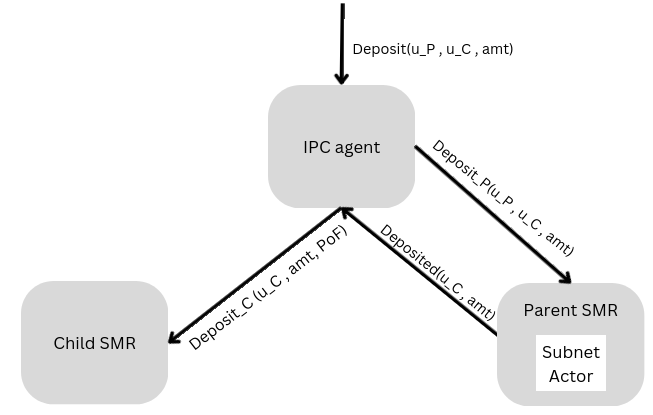
\includegraphics[width=\textwidth]{deposit}
%      \caption{Events produced and consumed during a deposit.}
%      \label{fig:deposit}
% \end{figure}
 

\begin{algorithm}[H]
\footnotesize
\caption{Deposit operation}\label{alg:deposit}
  \DontPrintSemicolon
  \SetKwFunction{FMain}{Global}
  \SetKwProg{Pn}{Function}{:}{\KwRet}
  \SetKwInOut{Input}{input}
  \SetKwProg{Component}{$\blacktriangleright$ \bf}{:}{\KwRet}
  \SetKwFor{UponKW}{upon}{do}{fintq}
  \del{\Input{\src account in parent, \dest account in child, amount~$\fil$}}
   \Component{\replace{IPC agent}{Owner of \src}}{
        submit $\tx=\textit{\add{P.\sa.}Deposit}\left( \src, \fil, \del{\sa.\textit{accounts}.}\dest \right)$ to parent \replace{\smr replica}{subnet}\;
  }
   \Component{\replace{Parent \smr replica}{P.\sa.Deposit(\src, amt, \dest)}}{
    move $\fil$ from \src to \add{P.}\sa.\textit{accounts}.\dest  \tcp*[r]{"lock" at parent}
    \del{notify agent \texttt{ParentDeposited}(\tx)}
  }
  \Component{IPC agent}{
    \UponKW{\replace{notification of \texttt{ParentDeposited}(\tx) from parent \smr}{tx = P.\sa.Deposit final at parent}}{
        create \prf that \tx is final at parent \smr \tcp*[r]{see \cref{sec:finality} for details}
        submit \replace{\texttt{Deposited}$=\langle \tx, \prf \rangle$ to child \smr}{\textit{P/C.\gw.Deposited(amt, \dest, \pof)}}
     }
  }
  \Component{\replace{Child \smr replica}{P/C.\gw.Deposited(amt, \dest, \pof)}}{
%    \UponKW{\texttt{Deposited}}{
        \replace{assert \gw.\verifyPfinal{\tx}{\prf}}{verify(\pof)}\;
        increase \dest account by \fil
%     }
  }
\end{algorithm}
\del{
One thing that differs a downward transaction (e.g., deposit) from an upward transaction (e.g., checkpoint) is that any participant that operates the child \smr replica also has visibility into the state of the parent \smr (albeit stale) through its local parent \smr replica. This enables the \textbf{local validity check} method to assert the finality at the parent (which may or may not be preferred over others).%
\footnote{\textbf{local validity check} (simpler, efficient, \textit{weaker guarantees}): $\prf$ contains a pointer to the block containing \tx  at the parent, together with the height~$h$ of that block.
 To assert that \tx is final, the child queries the parent about $\tx$, if it exists -- return valid, else -- return invalid. If invalid but the parent is still below height~$h$, then query again when parent reaches height~$h$.
This is a test inside the child \smr process. Therefore, if we want this method (and I believe we do), we should widen the interface so that a child \smr can ask the agent to get data from the parent. However, this optimization comes at the expense of the encapsulation of components, that is, it entails tinkering with the child \smr code.}
}

\subsection{Withdrawals}
\label{sec:withdraw}

A withdrawal is a transfer of funds from \replace{a user $\user$ account in the child subnet to $\user$'s account in the parent subnet. We assume that $\user$ is a participant running a parent replica, a child replica and an \ipc agent.}{an account \src in the child subnet $P/C$ to an account \dest in the parent subnet $P$}.
The \replace{withdraw}{\emph{Withdraw}} is performed \replace{as follows}{analogously to the \emph{Deposit}, but starting at the child subnet $P/C$}:
\begin{enumerate}
  \item \replace{$\user$ triggers the}{The owner of \src submits a transaction \emph{tx =}} $\textit{\add{P/C.\gw.}Withdraw}(\src, \fil, \dest)$\del{ operation at the local \ipc agent}.
    \del{\item The local \ipc agent submits the corresponding (properly signed) transaction $\tx = \textit{Withdraw}(\src, \fil, \dest)$ to the child SMR replica.}
    \item The child \replace{SMR system}{subnet} orders and executes the \emph{Withdraw} transaction, burning $\fil$ funds in \del{$\user$'s account} $\src$ (provided $\src$ has enough funds).
    \item When the child's replicated state that includes the transaction becomes final (for some SMR-system-specific definition of finality that has been defined in the SA), the \replace{local child replica notifies the local \ipc agent, potentially attaching a proof \prf that this state is final}{\ipc agent constructs a corresponding \pof and submits a transaction \textit{\tx' = P.\sa.Withdrawn(\fil, \dest, \pof)} to the parent subnet}.
    \del{\item The \ipc agent constructs a transaction $\tx' = \texttt{Burned}(\src, \fil, \dest, \prf)$ and submits it to the parent SMR system}.
    \item Upon ordering $\tx'$, \replace{the replicated logic of the parent SMR system updates the state of the \sa transferring the funds}{\emph{P.\sa.Withdrawn(amt, \dest, \pof)} verifies the \pof and transfers \emph{amt}} from \sa (concretely, to $\src$ account representation within the \sa) to \del{$\user$'s account} $\dest$ \add{within the parent subnet}.
\end{enumerate}

 % \begin{figure}[h]
 %     \centering
 %     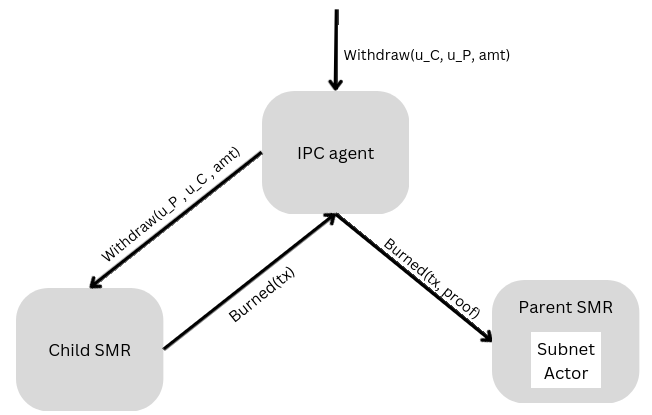
\includegraphics[width=\textwidth]{withdrawal}
 %     \caption{Events produced and consumed during a withdrawal.}
 %     \label{fig:withdrawal}
 % \end{figure}
\begin{algorithm}[H]
\footnotesize
\caption{Withdraw operation}\label{alg:withdraw}
  \DontPrintSemicolon
  \SetKwFunction{FMain}{Global}
  \SetKwProg{Pn}{Function}{:}{\KwRet}
  \SetKwInOut{Input}{input}
  \SetKwProg{Component}{$\blacktriangleright$ \bf}{:}{\KwRet}
  \SetKwFor{UponKW}{upon}{do}{fintq}
  % \Input{user~$\user$, amount~$\fil$, transaction \txnf}
   \del{\Input{\src account in child, \dest account in parent, $\fil$ amount of coins}}
   \Component{\replace{IPC agent}{owner of \src}}{
        submit $\tx=\textit{\add{P/C.\gw.}Withdraw}(\src, \fil, \dest)$\del{ to child \smr}\;
  }
   %
   \Component{\replace{Child \smr replica}{\textit{\add{P/C.\gw.Withdraw}(\src, \fil, \dest)}}}{
   \UponKW{$\tx = \textit{Withdraw}(\src, \fil, \dest)$}{
    deduct $\fil$ from \src \del{account at child} \tcp{"burns" \fil in child}
    \del{notify agent \texttt{Burned}(\tx)}
   }
  }
  \Component{IPC agent}{
    \UponKW{\replace{notification of \texttt{Burned}(\tx) from child \smr replica}{tx = P/C.\gw.Withdraw(\src, \fil, \dest)} final at child}{
        create \replace{\prf that \tx is final at child \smr}{$\pof(tx)$} \tcp*[r]{see \cref{sec:finality} for details}
        submit \replace{$\tx'=\texttt{Burned}\left(\tx, \prf \right)$  to parent \smr replica}{\textit{P.\sa.Withdrawn(amt, \dest, \pof)}}
     }
  }
  \Component{P.\sa.Withdrawn(amt, \dest, \pof)}{
    \replace{assert \sa.\verifyGfinal{\prf}{\tx}}{verify($\pof(tx')$)}\;
    move \fil coins from \add{P.}\sa\del{.\textit{accounts}.\src} to \dest \tcp{"unlocks" \textit{amt} for \dest}
  }
   
%    \Component{Child SMR}{
%    [\tx submitted by user, proposed, written]\\
%    \UponKW{\txnf written in Child SMR}{
%     decrease user fund's by $\fil$\\
%     Send \texttt{ChildWithdrawn(\tx, [$proof$])} to IPC agent \tcp*[r]{notify IPC agent}
%    }
%   }
%   \Component{IPC agent}{
%     \UponKW{\texttt{ChildWithdrawn(\tx, [$proof$])} notified by Child SMR}{
%     \If{$proof=$ \textbf{nil}}{
%          $proof \gets $\textit{generateProofOfGlobalFinality(\tx,...)} \tcp*[r]{Necessary steps for \tx to be ready to be submitted to Parent SMR}
%      }
%      \texttt{ChildWithdrawn(\tx, $proof$)} to parent SMR \tcp*[r]{Submit to parent}
%      }
%     \UponKW{\arp{State updated after Withdrawal}}{ \tcp*[r]{Notified when parents update state}
%       \arp{Check child subnet rules are still satisfied, remedy/close otherwise?}
%     }
%   }
%   \Component{Parent SMR}{
%   \UponKW{\texttt{ChildWithdrawn(\tx, $proof$)} submitted by IPC agent}{
%       \If{\sa.\verifyGfinal{\tx}{\prf}}{
%            [tx submitted by IPC agent, proposed, written]\\
%            \UponKW{\txnf written in Parent SMR}{
%                 reduce $\fil$ amount for user $\user$ in SA\\
%                 Parent SMR notifies IPC agent
%             }
%       }
%   }
% }
\end{algorithm}
\label{enhancedFunc}

\subsection{Checkpointing} 
A checkpoint contains a representation of the \del{updated} state of the child \replace{SMR system}{subnet} to be included in the parent \replace{SMR system}{subnet's replicated state}. A checkpoint can be triggered by predefined events (i.e. periodically after a number of state updates, triggered by a specific user or set of users, etc.). \del{As such, the checkpoint functionality may or may not be triggered by a user request on the child SMR.} A checkpoint is \replace{performed}{created} as follows:
\replace{
\begin{enumerate}
\item When the predefined checkpoint trigger is met (the IPC Agent, monitoring the child subnet's state, is configured with the checkpint trigger), the IPC agent queries the parent's \sa.
\item If the participant is a validator according to \sa's state, then the IPC agent queries the child SMR replica for the child's state to be represented in this checkpoint. 
\item The IPC agent creates a \prf that this updated state of the child SMR system is final, possibly compressing its representation of the state. 
\item The IPC agent evaluates a function \ssc(sa, parent's state, etc.) and decides whether the participant submits the checkpoint. If the function returns true, then the IPC agent submits a transaction $\tx=\texttt{Checkpoint}\left(\textit{state}, \prf \right)$ to the parent SMR replica.
 \item Upon ordering $\tx$, the replicated logic of the parent SMR system updates the state of the SA according to the checkpoint state, if necessary.
\end{enumerate}
}{
\begin{enumerate}
    \item When the predefined checkpoint trigger is met (the IPC Agent, monitoring the child subnet's state, is configured with the checkpint trigger),
    the IPC agent retrieves the corresponding chackpoint data (\emph{chkp}) from the child subnet, along with the proof of its finality (\emph{\pof}).
    \item \TODO{Here the IPC Agent should decide (based on some possible reward) whether to submit the Checkpoint transaction.}
    \item The IPC agent submits a transaction \emph{tx = P.\sa.Checkpoint(chkp, \pof)}.
    \item The\emph{P.SA.Checkpoint(chkp, \pof)} invocation, after verifying the \emph{\pof}, includes \emph{chkp} in its state.
\end{enumerate}
}

\TODO{Pseudocode}
% See commented algorithm

% \begin{figure}[h]
%      \centering
%      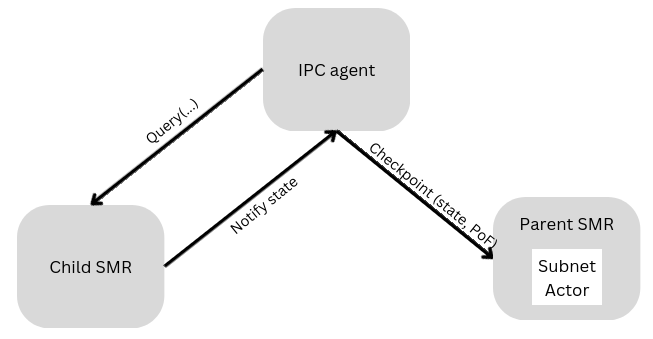
\includegraphics[width=\textwidth]{checkpoint.png}
%      \caption{Events produced and consumed by the checkpointing functionality.}
%      \label{fig:chkp}
%  \end{figure}
% \begin{algorithm}[H]
% \footnotesize
% \caption{Checkpoint operation}\label{alg:down}
%   \DontPrintSemicolon
%   \SetKwFunction{FMain}{Global}
%   \SetKwProg{Pn}{Function}{:}{\KwRet}
%   \SetKwInOut{Input}{input}
%   \SetKwProg{Component}{$\blacktriangleright$ \bf}{:}{\KwRet}
%   \SetKwFor{UponKW}{upon}{do}{fintq}
%    \Component{IPC agent}{
%         \If{trigger for checkpoint}{
%             \textit{SA\_state} $\gets$ query parent for \sa's state\;
%             \If{\textit{Self} \textbf{in} SA\_state.validators}{
%                 \textit{state} $\gets$ query child for state\;
%                 \textit{cState} $\gets$ \textit{compressState}(\text{state},\textit{SA\_state.latestCheckpoint})\;
%                 create \prf that \textit{cState} is final at child\;
%             }
%             $\tx=\sa.\texttt{Checkpoint}\left(\textit{cState}, \prf \right)$ \;
%             \If{\textit{Self.}\ssc(tx, SA\_state, ...)}{
%                 submit $tx$ to parent \smr replica\;
%             }
%         }
%   }
%   \Component{parent \smr replica}{
%     \UponKW{$\tx=\sa.\texttt{Checkpoint}\left(\textit{cState}, \prf \right)$}{
%         assert \sa.\verifyGfinal{\textit{cState}}{\prf}\;
%         $\sa.\textit{latestCheckpoint.update}(\textit{cState})$
%      }
%   }
% \end{algorithm}
The above pseudo code is intentionally abstract, with a number of implementation decisions not specified, such as the main function for creating and verifying a \prf, events that trigger the creation of a new checkpoint, the compression procedure with respect to the previous checkpoint, and the \ssc function to decide whether the participant submits or not a checkpoint. 

% The above pseudo code is highly abstract, with the main function of creating and verifying a \prf not specified. Moreover, other important aspects that are not covered include specific compression mechanisms for the checkpoint data, triggering checkpoints efficiently, and particular incentives for checkpoints creation and submission. \arp{we refer to reference implementation... later in this document we list others...}
% The function \ssc comprises two aspects of the checkpointing functionality from the perspective of participants. First, it controls access to submit checkpoints, as not all subnets will define the same policy to follow when deciding the participants that are allowed to submit checkpoints. Second, it contains the implications of submitting a checkpoint transaction (i.e. the cost involved in being the submitter). For example, if only one transaction is required by any participant but the cost of submitting the checkpoint is incurred on the submitter, then there is a risk of no participant actually submitting the checkpoint if they are strictly rational. An example on the other end might be requiring all participants to submit a transaction for the checkpoint to be finalized at the parent, but this approach affects performance. \arp{We analyze and suggest later in this document multiple mechanisms to ensure through incentives that at least one rational participant will always submit the checkpoint. }

\subsection{Slashing} 
\guy{This section is immature for review (even a preliminary one)}\\
We show here the events produced and consumed by the slashing functionality. Given specific misbehavior from participants that is identified as Proofs of Fraud (PoFs), e.g.
gathering signed equivocating messages, the child SMR reports the PoFs to the IPC agent, which immediately forwards a slash a request to the parent SMR. \arp{Extend with need to verify if child SMR can continue, needs to remedy its depleted collateral or should be killed with latest checkpoint/state update}.
% \begin{figure}[h]
%      \centering
%      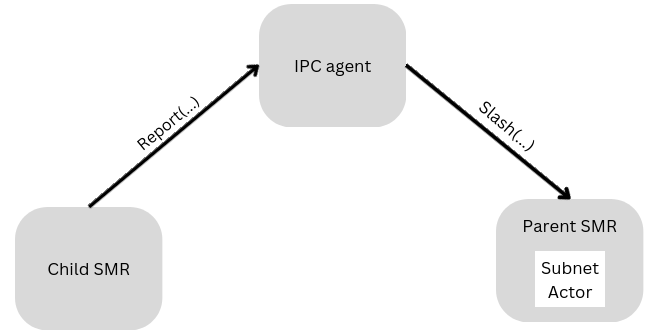
\includegraphics[width=\textwidth]{slash}
%      \caption{Events produced and consumed by the slashing functionality.}
%      \label{fig:report}
%  \end{figure}\\

\begin{algorithm}[H]
\footnotesize
\caption{Slash Functionality}\label{alg:down}
  \DontPrintSemicolon
  \SetKwFunction{FMain}{Global}
  \SetKwProg{Pn}{Function}{:}{\KwRet}
  \SetKwInOut{Input}{input}
  \SetKwProg{Component}{$\blacktriangleright$ \bf}{:}{\KwRet}
  \SetKwFor{UponKW}{upon}{do}{fintq}
  \Input{-}
  \Component{Child SMR}{
     \UponKW{Proofs of fraud \pofs generated}{
       Notify \report to IPC agent
     }
  }
  \Component{IPC agent}{
    \UponKW{\report notified by child SMR}{
        Submit \slashop to parent SMR
    }
    \UponKW{\arp{State updated after slashing}}{
      \arp{Check child SMR rules are still satisfied, remedy/close otherwise?}
    }
  }
  \Component{Parent SMR}{
        \UponKW{\slashop submitted by IPC agent}{
         Update SA state slashing/excluding participants
         Notify SA update to IPC agent
        }
  }
\end{algorithm}


\subsection{Propagating cross-net transactions}
\replace{The \postoffice functionality is an inter-subnet transaction service. The main motivation for this functionality comes from a ``potential clients" request: enable a \dapp in one subnet to interact with a \dapp in a different subnet.}{
\matej{This section is in a preliminary stage, take with a grain of salt.}
}

\add{
The implementation of the Gateway Actor's \emph{Propagate} function is sketched in \Cref{alg:po}
}
% \guy{Edge case: a leaf subnet does not have a \sa and, therefore, no \postoffice. We can consider removing the \postoffice functionality from the \sa and to deploy it as an independent \dapp that will appear only once per subnet. In this case, it needs permissions to call \sa.\verifyGfinal{\tx}{\prf} function.}

\begin{algorithm}[H]
\footnotesize
\caption{Cross-net transaction propagation functionality}\label{alg:po}
  \DontPrintSemicolon
  \SetKwFunction{FPropagate}{propagate}
  \SetKwProg{Pn}{Function}{:}{\KwRet}
  \SetKwInOut{Input}{input}
  \SetKwProg{Component}{$\blacktriangleright$ \bf}{:}{\KwRet}
  \SetKwProg{Empty}{\bf}{:}{\KwRet}
  \SetKwFor{UponKW}{upon}{do}{fintq}
  \del{\Input{$\tx = \langle \data, \src, \dest, \prf \rangle$}}
  \Component{\gw.Propagate($\tx = (\data, \src, \dest, \prf)$)}{
    verify(\tx.\pof)
    \Case{\dest in current subnet}{
        \propagate\textit{HERE}(\tx)
    }
    \Case{\dest requires going up the tree}{
        \propagate\textit{UP}(\tx)
    }
    \Case{\dest requires going down the tree}{
        \propagate\textit{DOWN}(\tx)
    }
  }
  % \Component{parent \smr process}{
  %    \UponKW{event \postoffice.UP$\langle \data, \src, \dest \rangle$}{
  %       $\tx \gets \langle \data, \src, \dest \rangle$\;
  %       notify agent on \postoffice.UP(\tx)
  %    }
  % }
  \Component{PropagateUP(tx)}{
    Add transaction \emph{tx' = parent.\gw.Propagate((data, src.(this\_subnets\_name), dest))} to the list of cross-net transactions (to be noticed and submitted by the IPC agent)
       % \src.\textit{append(\gw's subnet id)}\tcp*[r]{the i.d. of the current subnet}
       % Add updated transaction \gw.\postoffice.UP$\langle \data, \src, \dest \rangle$

  }
 \tcp{\propagate\textit{DOWN}(\tx) is analogous to \propagate\textit{UP}(\tx)}
 \tcp{\propagate\textit{HERE}(\tx) is trivial}
  \Component{IPC agent}{
    \UponKW{new transaction tx' in the list of cross-net transactions}{
        Create \pof proving that \tx' has indeed been added to the list fo cross-net transactions in the subnet\;
        submit \tx', augmented by \emph{\pof}
    }   
}
\end{algorithm}

% OLD PSEUDOCODE
% \begin{algorithm}[H]
% \footnotesize
% \caption{\postoffice Functionality}\label{alg:po}
%   \DontPrintSemicolon
%   \SetKwFunction{FPropagate}{propagate}
%   \SetKwProg{Pn}{Function}{:}{\KwRet}
%   \SetKwInOut{Input}{input}
%   \SetKwProg{Component}{$\blacktriangleright$ \bf}{:}{\KwRet}
%   \SetKwProg{Empty}{\bf}{:}{\KwRet}
%   \SetKwFor{UponKW}{upon}{do}{fintq}
%   \Input{$\tx = \langle \data, \src, \dest, \prf \rangle$}
%   \Component{\gw.\postoffice}{
%      \UponKW{\postoffice.\propagate(\tx) }{
%        \Case{\dest in current subnet}{
%             \postoffice.\propagate\textit{HERE}(\tx)
%        }
%        \Case{\dest requires going up the tree}{
%             \postoffice.\propagate\textit{UP}(\tx)
%        }
%        \Case{\dest requires going down the tree}{
%             \postoffice.\propagate\textit{DOWN}(\tx)
%        }
%      }
%      \UponKW{\postoffice.\propagate\textit{UP}(\tx) }{
%        \If{\src not from this subnet}{
%             assert \sa.\verifyGfinal{\tx}{\prf}\tcp*[r]{the \sa that corresponds to the child subnet from which \tx comes}
%        }
%        \src.\textit{append(\gw's subnet id)}\tcp*[r]{the i.d. of the current subnet}
%        emit event \gw.\postoffice.UP$\langle \data, \src, \dest \rangle$\;
%        % $\tx \gets \langle \data, \src, \dest \rangle$\;
%        notify agent on \gw.\postoffice.UP$\langle \data, \src, \dest \rangle$
%      }
%      \tcp{\propagate\textit{DOWN}(\tx) is analogous to \propagate\textit{UP}(\tx)}
%      \tcp{\propagate\textit{HERE}(\tx) is trivial}
%   }
%   % \Component{parent \smr process}{
%   %    \UponKW{event \postoffice.UP$\langle \data, \src, \dest \rangle$}{
%   %       $\tx \gets \langle \data, \src, \dest \rangle$\;
%   %       notify agent on \postoffice.UP(\tx)
%   %    }
%   % }
%   \Component{IPC agent}{
%     \UponKW{notification of \gw.\postoffice.UP$\langle \data, \src, \dest \rangle$ from child}{
%         $\tx' \gets$ \gw.\postoffice.UP$\langle \data, \src, \dest \rangle$\;
%         create \prf that \tx' is final at child \smr\;
%         $\tx_\textit{new}\gets\langle \tx', \prf \rangle$\;
%         submit \gw.\postoffice.\propagate($\tx_\textit{new}$) to parent \smr
%     }   
% }
% \end{algorithm}
% \subsection{Atomic Execution}
% TODO
